\chapter{Sprint 5 : pilotage, déploiement et recette}
\label{ch:sprint5}
\startcontents[chapters]
\chapterplan

\section{Introduction}

Les quatre premiers sprints ont livré les fonctions de la plateforme : sécurité et administration, saisie des fiches, génération et validation des fichiers SEPA, détection intelligente d'anomalies. Le dernier sprint a un autre objet : rendre cet ensemble \textbf{pilotable}, \textbf{reproductible} et \textbf{vérifié}. Il répond à trois questions. Que doit voir chaque profil dès son arrivée dans l'application ? Comment une autre équipe peut-elle installer la plateforme sans reconstituer à la main chaque composant ? Et comment s'assurer que l'ensemble, et non seulement chaque fonction isolée, se comporte comme les chapitres précédents l'annoncent ? Planifié sur quatre semaines (tableau~\ref{tab:sprints}), le sprint couvre les récits US21 à US24 (tableau~\ref{tab:backlog}). Ce chapitre présente les tableaux de bord et les indicateurs, le déploiement par conteneurs, la documentation de l'API, puis la recette de bout en bout menée sur l'application déployée.

\section{Conception}

La figure~\ref{fig:uc-s5} présente les cas d'utilisation du sprint. Les trois profils consultent un tableau de bord et les indicateurs, avec un contenu propre à chacun. L'équipe technique, qui n'est pas un profil de l'application mais l'acteur du déploiement et de la recette, installe la plateforme, consulte la documentation de l'API et déroule la recette.

\begin{figure}[H]
\centering
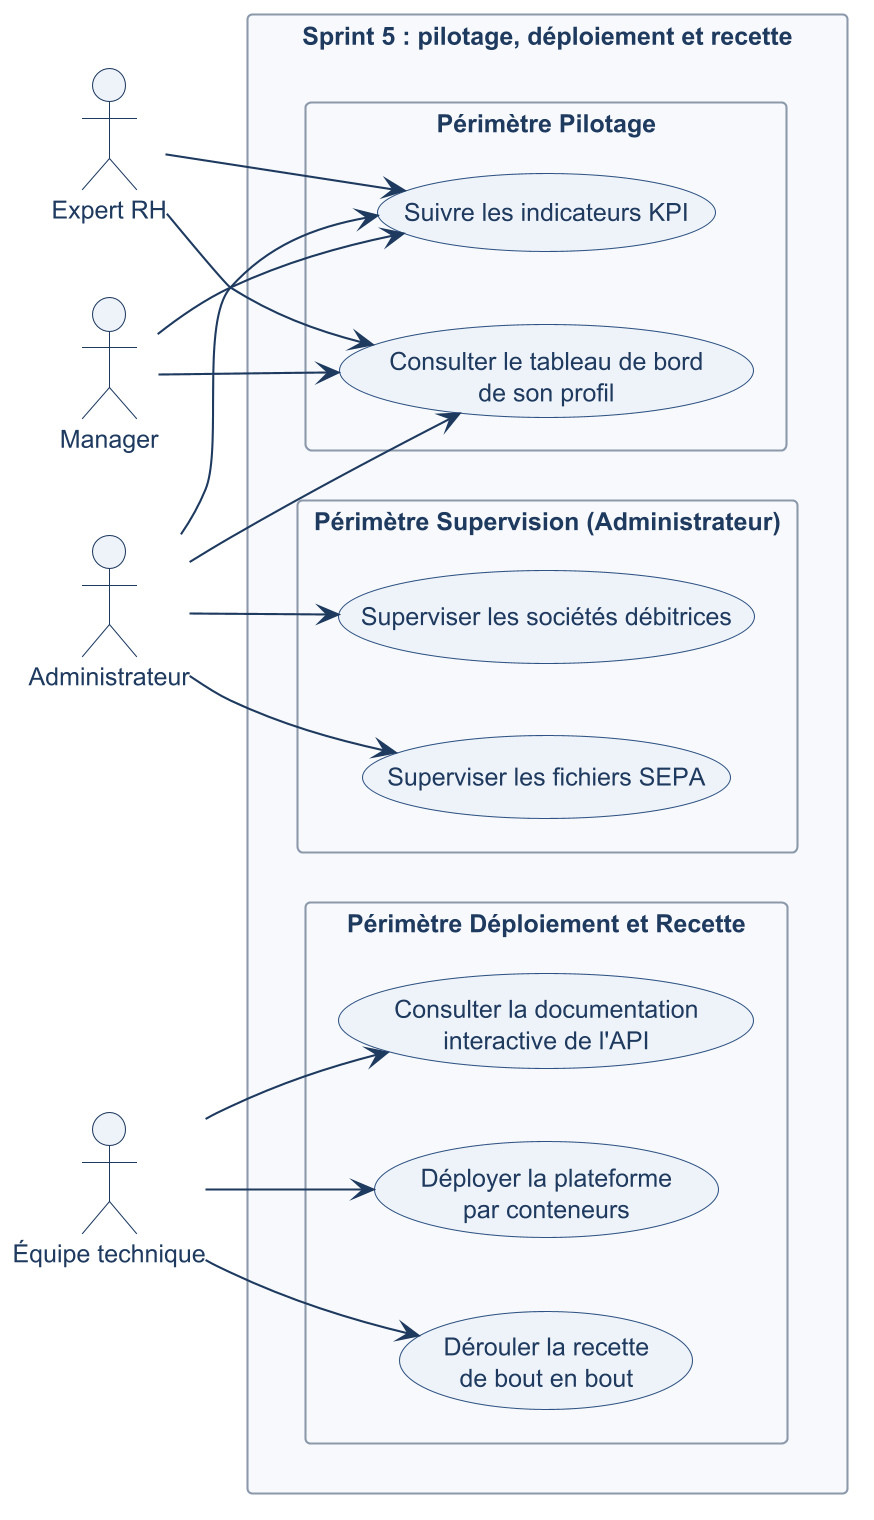
\includegraphics[height=0.34\textheight,width=\textwidth,keepaspectratio]{fig8_1_cas_utilisation_sprint5}
\caption{Cas d'utilisation du sprint 5}
\label{fig:uc-s5}
\end{figure}

Deux principes guident la conception des tableaux de bord. Le premier est celui d'un \textbf{écran orienté action} : un Expert RH ou un Manager n'ouvre pas l'application pour lire des statistiques, mais pour savoir ce qui l'attend. Le tableau de bord présente donc d'abord ce qui demande une action, puis, séparément, les chiffres du mois. Le second est le \textbf{respect du cloisonnement} défini au chapitre~\ref{ch:besoins} : chaque profil ne reçoit que les données auxquelles il a droit, et ce filtrage est appliqué par le serveur, non par l'interface.

\section{Tableaux de bord}

\subsection{Un contenu adapté à chaque profil}

Le tableau de bord se compose de deux blocs. Le bloc \og À traiter maintenant\fg{} compte, à la date du jour, les éléments qui attendent une action ; le bloc \og Ce mois-ci\fg{} résume l'activité du mois en cours. Les cartes du premier bloc renvoient vers l'écran qui permet de traiter l'élément. Le contenu diffère selon le profil (tableau~\ref{tab:dashboard-profils}).

\begin{table}[H]
\centering
\footnotesize
\renewcommand{\arraystretch}{1.15}
\tablestyle
\begin{tabularx}{\textwidth}{|>{\raggedright\arraybackslash}p{2.6cm}|Y|Y|}
\hline
\rowcolor{appMarine}\entete{Profil} & \entete{À traiter maintenant} & \entete{Ce mois-ci} \\
\hline
Expert RH & Fichiers rejetés à corriger ; fichiers à soumettre ; anomalies ouvertes ; transactions à approuver et rejetées & Fiches approuvées ; fichiers générés et part validée ; taux d'erreur. Aucun montant \\
\hline
Manager & Fichiers à valider ; anomalies ouvertes ; transactions à approuver et rejetées & Fiches approuvées ; fichiers générés et part validée ; taux d'erreur \\
\hline
Administrateur & Supervision des fichiers : en attente de validation, rejetés, non conformes au schéma XSD & Fiches approuvées ; fichiers générés ; taux d'erreur ; montant ; tableau par société. Aucune donnée individuelle \\
\hline
\end{tabularx}
\caption{Contenu du tableau de bord selon le profil}
\label{tab:dashboard-profils}
\end{table}

Les cartes sont colorées selon l'urgence : un compteur nul s'affiche en vert avec la mention \og Rien à traiter\fg{}, un élément en attente en orange, un rejet ou une anomalie en rouge. La figure~\ref{fig:dash-expert} présente la vue de l'Expert RH sur le jeu de démonstration du chapitre~\ref{ch:sprint4} ; celle du Manager a la même structure et porte sur toutes les sociétés. Le montant global des paiements n'apparaît pas pour l'Expert RH, conformément à la séparation des rôles.

\begin{figure}[H]
\centering
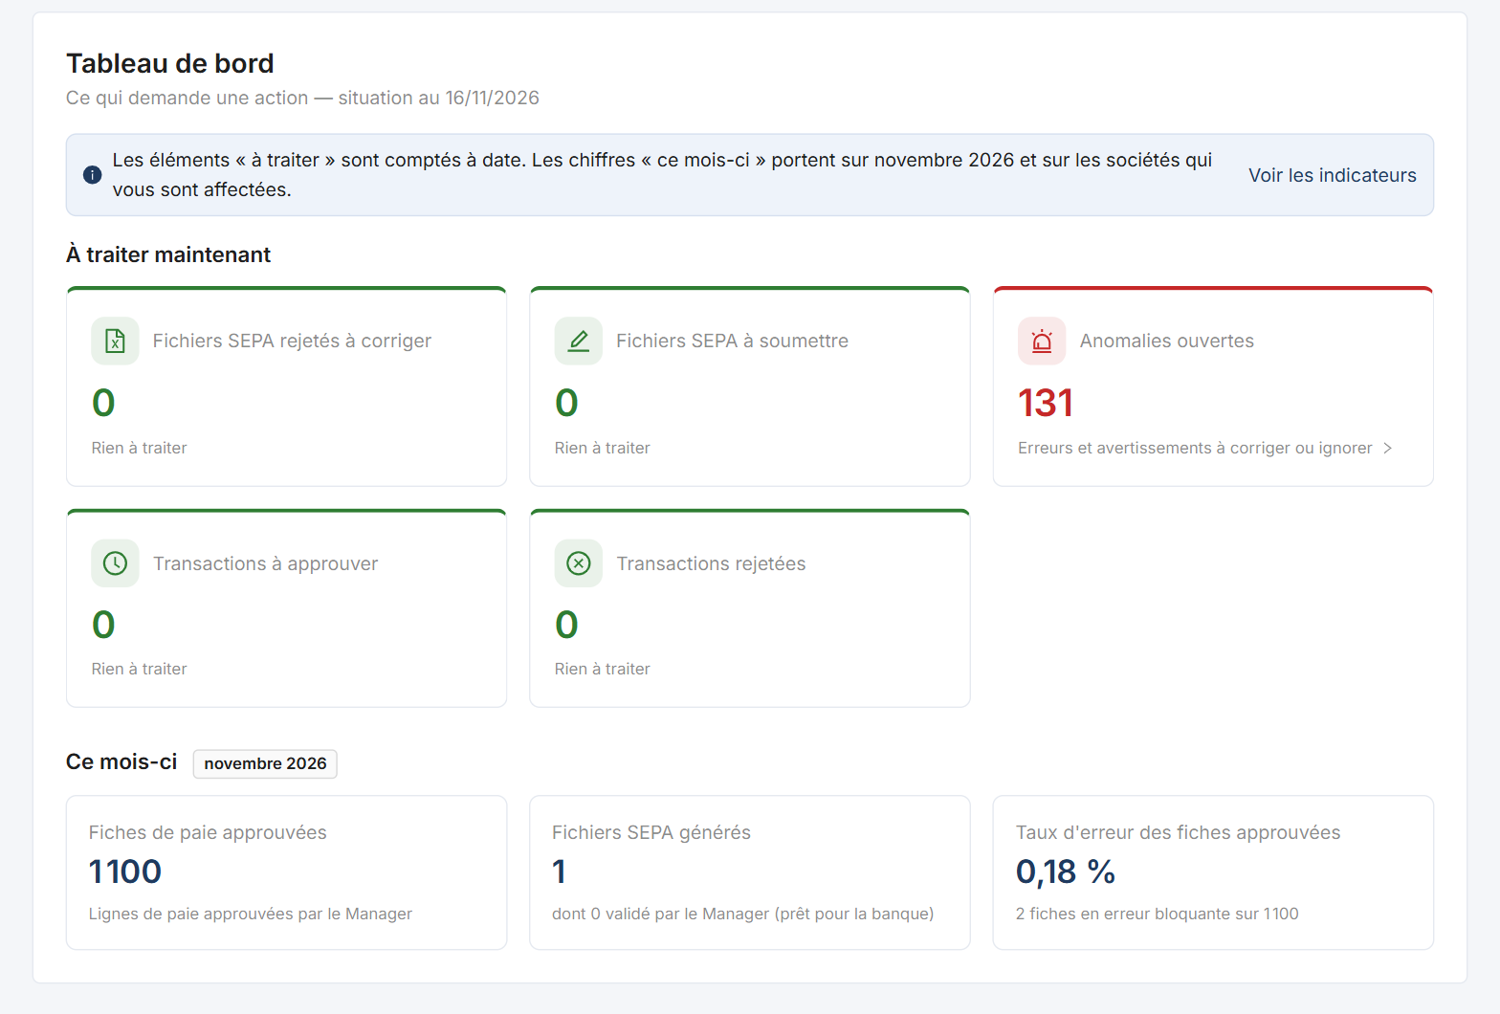
\includegraphics[width=0.85\textwidth]{fig8_dashboard_expert}
\caption{Tableau de bord de l'Expert RH (périmètre limité à ses sociétés affectées)}
\label{fig:dash-expert}
\end{figure}

\subsection{Périmètre de l'Expert RH et supervision de l'administrateur}

Les chiffres de l'Expert RH reposent sur les fiches, les fichiers et les anomalies de ses seules sociétés affectées : la liste des fiches, l'analyse à la demande et le registre des anomalies, y compris la modification du statut d'une anomalie, sont limités à son périmètre, et un Expert RH sans société affectée ne voit aucune fiche ni aucune anomalie. Ce filtrage a été complété à la suite de la recette décrite plus loin, qui avait montré que les anomalies de toutes les sociétés étaient encore comptées.

L'administrateur dispose d'une vue de supervision (figure~\ref{fig:dash-admin}). Elle indique combien de fichiers attendent la validation du Manager, combien ont été rejetés et combien ne sont pas conformes au schéma XSD, ainsi que les totaux du mois et un tableau par société. Ce tableau cumule le \textbf{montant des fichiers SEPA générés} (un salarié y est compté une fois par fichier), à distinguer du \textbf{montant des fiches approuvées} du mois : le premier porte sur les fichiers produits, le second sur les fiches validées par le Manager. Cette vue ne contient aucune donnée individuelle de paie : l'administrateur surveille le fonctionnement du système sans accéder aux salaires.

\begin{figure}[H]
\centering
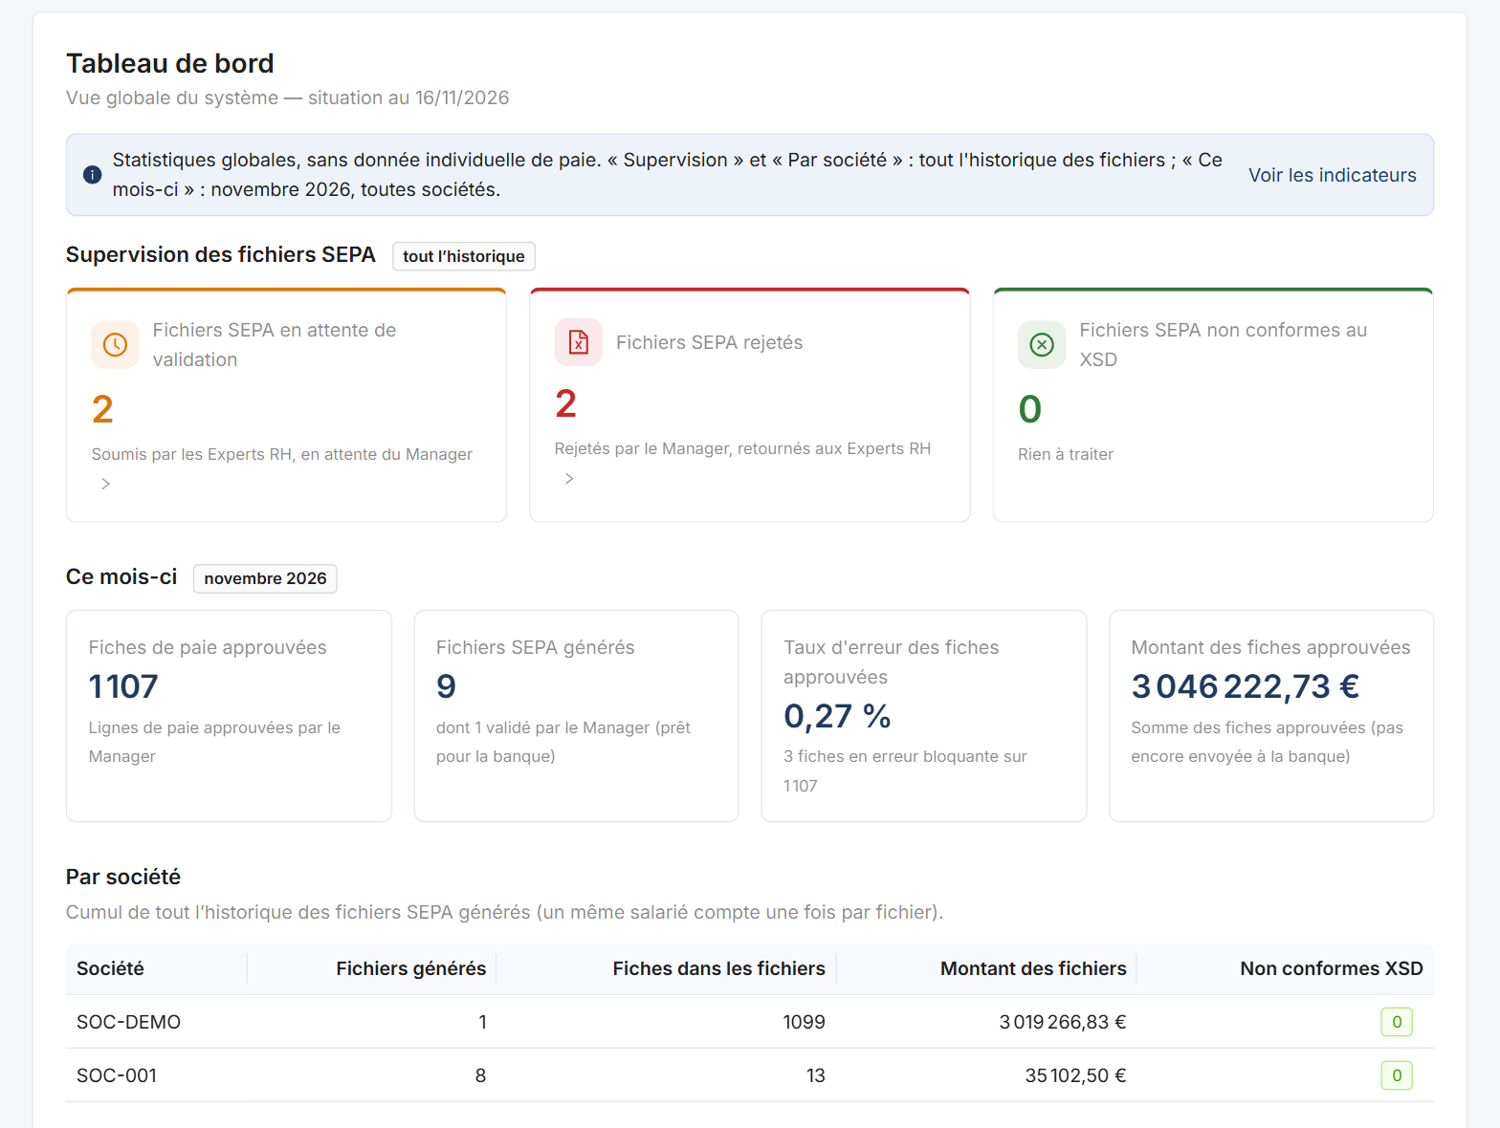
\includegraphics[width=0.9\textwidth]{fig8_dashboard_admin}
\caption{Tableau de bord de supervision de l'administrateur}
\label{fig:dash-admin}
\end{figure}

\section{Indicateurs de performance}

\subsection{Définitions et objectifs}

La page des indicateurs approfondit le tableau de bord sur une période et une société au choix. Son principe est qu'un indicateur n'a de valeur que s'il est défini sans ambiguïté. Chaque carte porte donc une définition, accessible au survol, et un encadré d'introduction rappelle la distinction essentielle entre une \textbf{fiche} (une ligne de paie, approuvée par le Manager) et un \textbf{fichier SEPA} (le XML créé à partir de fiches approuvées, soumis puis validé). Le tableau~\ref{tab:kpi} résume les indicateurs principaux.

\begin{table}[H]
\centering
\footnotesize
\renewcommand{\arraystretch}{1.15}
\tablestyle
\begin{tabularx}{\textwidth}{|>{\raggedright\arraybackslash}p{3.7cm}|Y|>{\centering\arraybackslash}p{1.8cm}|}
\hline
\rowcolor{appMarine}\entete{Indicateur} & \entete{Définition} & \entete{Objectif} \\
\hline
Taux d'approbation & Fiches approuvées par le Manager, rapportées à toutes les transactions du mois (hors supprimées) & $\geq$ 90~\% \\
\hline
Taux d'erreur des fiches approuvées & Fiches approuvées portant au moins une erreur bloquante non ignorée, rapportées aux fiches approuvées. Les avertissements ne comptent pas & $\leq$ 1~\% \\
\hline
Conformité XSD & Fichiers générés dont la validation XSD réussit, rapportés aux fichiers générés sur la période & $\geq$ 95~\% \\
\hline
Montant des fiches approuvées & Somme des montants approuvés ; ce n'est pas un montant transmis à la banque. Réservé au Manager et à l'administrateur & --- \\
\hline
Fiches approuvées, fichiers générés & Volumes de la période ; part des fichiers validés par le Manager & --- \\
\hline
Sociétés avec fiches approuvées & Sociétés distinctes ayant au moins une fiche approuvée & --- \\
\hline
Anomalies signalées & Anomalies de la période, réparties en ouvertes, corrigées et ignorées, avec la part d'erreurs bloquantes et d'avertissements & --- \\
\hline
Fiches signalées par l'IA ; part détectée par l'IA seule & Fiches suspectes selon la dernière analyse ; proportion de ces fiches que les contrôles métier ne signalent pas & --- \\
\hline
\end{tabularx}
\caption{Principaux indicateurs de la page KPI}
\label{tab:kpi}
\end{table}

Trois indicateurs sont assortis d'un objectif chiffré, et la couleur de leur carte traduit la situation : vert lorsque l'objectif est atteint, orange dans une zone intermédiaire, rouge au-delà. Ces seuils sont des cibles de pilotage fixées pour la démonstration ; ils devraient être arrêtés avec les futurs utilisateurs. Chaque carte affiche aussi l'écart avec le mois précédent, ce qui distingue une dégradation d'une situation stable.

La distinction entre erreur et avertissement mérite d'être soulignée. Un IBAN partagé entre deux salariés ou un montant jugé suspect par l'IA sont des signaux à vérifier, mais pas des fautes avérées : ils figurent dans le compte des anomalies, sans entrer dans le taux d'erreur. Ce choix évite qu'une alerte prudente de l'IA dégrade artificiellement la mesure de qualité.

\subsection{Lecture de la page}

La figure~\ref{fig:kpi} présente la page vue par le Manager. Au-dessous des cartes, un graphique donne l'évolution sur douze mois du nombre de fiches et du taux d'erreur, et deux représentations répartissent les anomalies par source (règles métier ou IA) et par type. L'Expert RH accède à la même page, limitée à ses sociétés, sans les montants globaux : un bandeau \og Vue limitée\fg{} le précise. Les chiffres de la figure sont ceux du jeu de démonstration et n'ont pas valeur de performance réelle.

\begin{figure}[H]
\centering
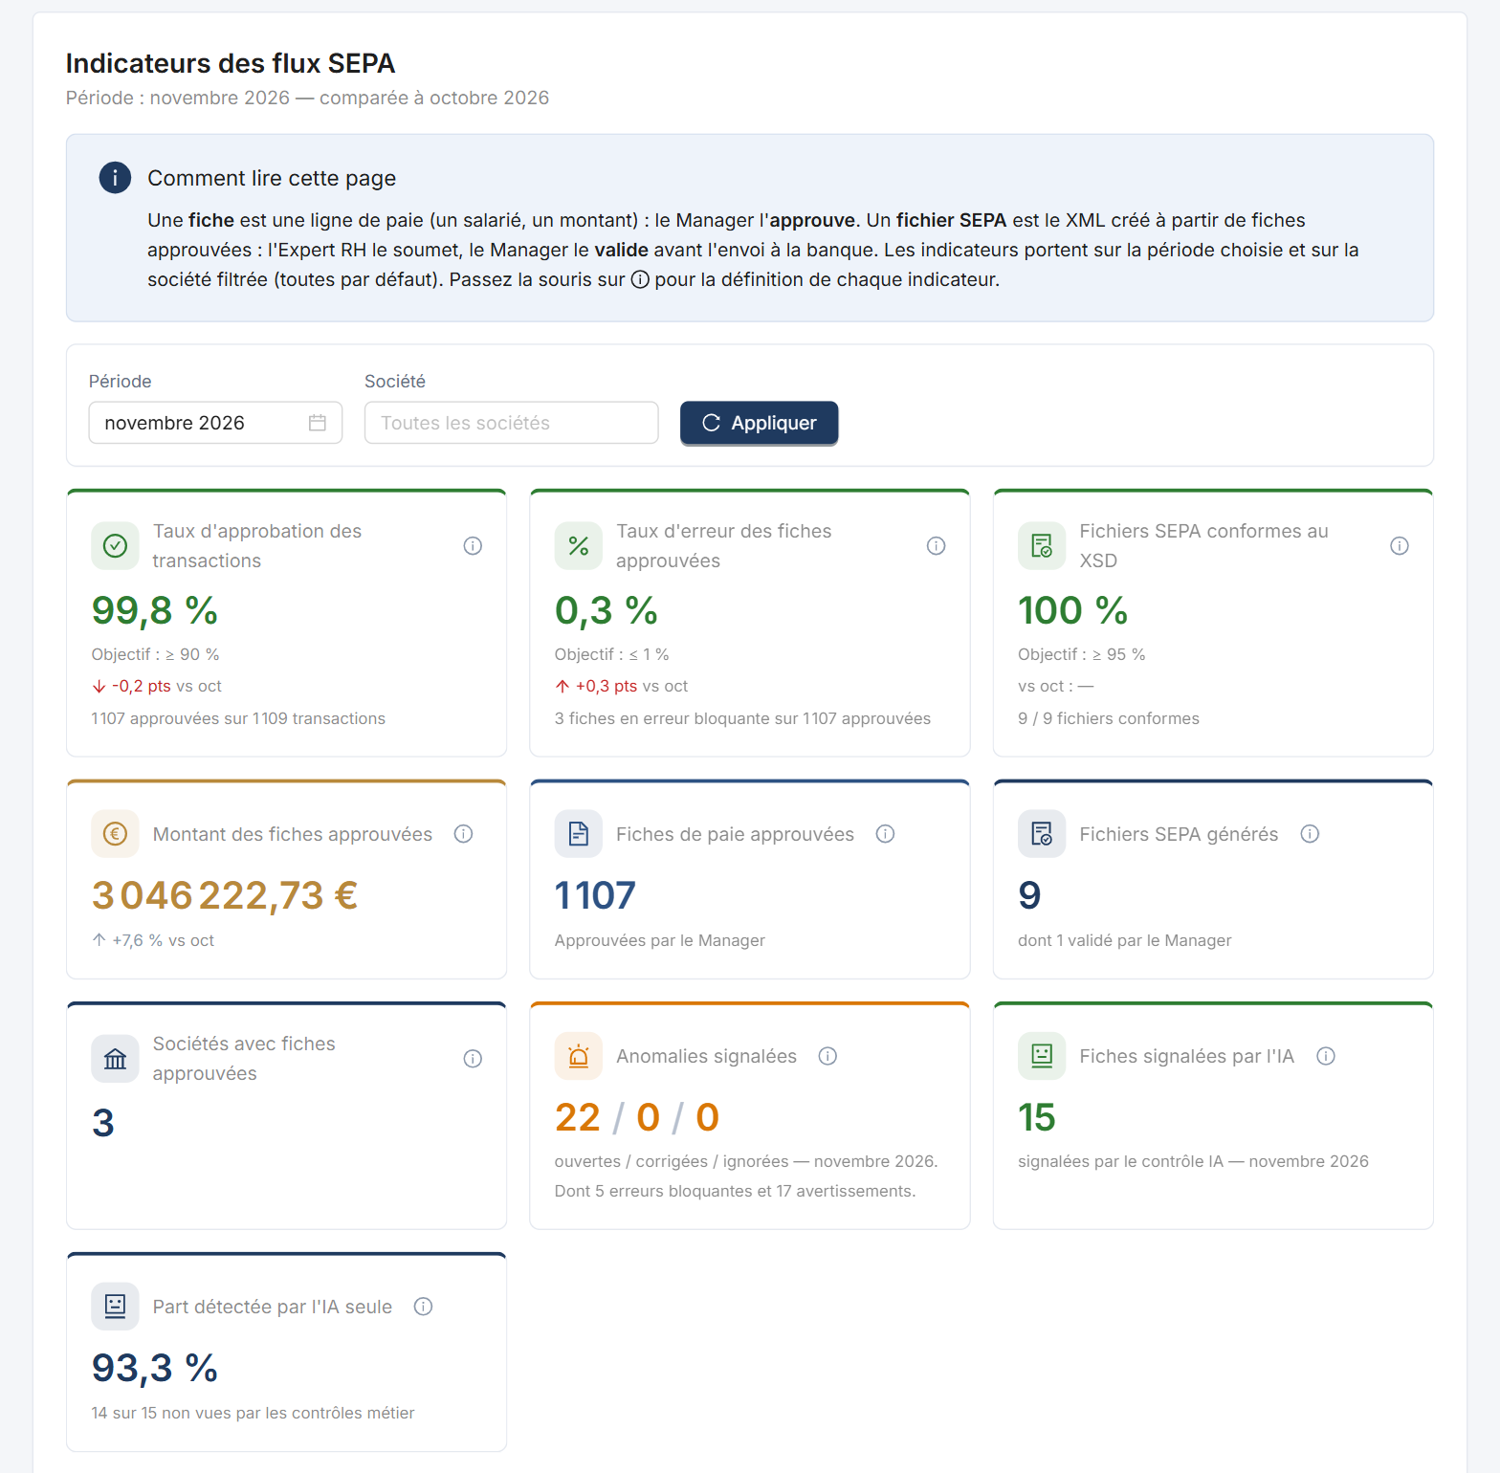
\includegraphics[height=0.66\textheight,width=0.85\textwidth,keepaspectratio]{fig8_kpi_manager}
\caption{Page des indicateurs vue par le Manager}
\label{fig:kpi}
\end{figure}

\section{Déploiement par conteneurs}

\subsection{Services et images}

La plateforme se déploie avec Docker Compose, qui décrit dans un seul fichier les cinq services de l'architecture présentée au chapitre~\ref{ch:architecture} : la base PostgreSQL, la messagerie de test MailHog, le module d'IA, le backend et l'interface web. Le tableau~\ref{tab:services} les récapitule avec leur origine et la taille de leur image.

\begin{table}[H]
\centering
\footnotesize
\renewcommand{\arraystretch}{1.15}
\tablestyle
\begin{tabularx}{\textwidth}{|>{\raggedright\arraybackslash}p{2.4cm}|Y|>{\centering\arraybackslash}p{1.5cm}|>{\centering\arraybackslash}p{1.8cm}|}
\hline
\rowcolor{appMarine}\entete{Service} & \entete{Contenu et origine de l'image} & \entete{Port} & \entete{Taille} \\
\hline
postgres & Image officielle PostgreSQL 16 ; volume de données persistant ; contrôle de santé & 5432 & 420~Mo \\
\hline
mailhog & Image officielle de messagerie de test (codes de connexion, notifications) & 8025 & 572~Mo \\
\hline
ai-module & Python 3.11, FastAPI et modèles de reconnaissance faciale téléchargés à la construction ; volume du modèle d'IA & 8000 & 1,02~Go \\
\hline
backend & Application Spring Boot construite en deux étapes : compilation avec Maven, puis exécution sur un environnement Java 17 allégé & 8080 & 371~Mo \\
\hline
frontend & Interface React compilée, puis servie comme ressources statiques & 5173 & 217~Mo \\
\hline
\end{tabularx}
\caption{Services déployés par Docker Compose}
\label{tab:services}
\end{table}

Les images du backend et de l'interface sont construites en \textbf{deux étapes}. La première contient les outils de compilation, la seconde uniquement ce qui est nécessaire à l'exécution : l'image finale ne transporte ni Maven ni les sources, ce qui la rend plus légère et réduit ce qu'elle expose. L'image du module d'IA est la plus volumineuse, car elle embarque l'environnement scientifique Python et les modèles de reconnaissance faciale.

\subsection{Configuration, ordre de démarrage et persistance}

La configuration est portée par des variables d'environnement : accès à la base, adresse du module d'IA, activation de l'IA, serveur de messagerie, exigence du code de connexion. Ainsi, la même image s'exécute dans des contextes différents sans être reconstruite.

Le démarrage respecte des dépendances : le backend n'est lancé qu'une fois la base déclarée saine par son contrôle de santé, et après le démarrage du module d'IA et de la messagerie ; l'interface attend le backend. Cet ordre évite qu'une application démarre sur une base qui n'accepte pas encore de connexions. La figure~\ref{fig:deploiement-local} distingue le navigateur des conteneurs : le conteneur de l'interface ne sert que les ressources de l'application, puis le code React s'exécute dans le navigateur, qui appelle directement l'API du backend.

\begin{figure}[H]
\centering
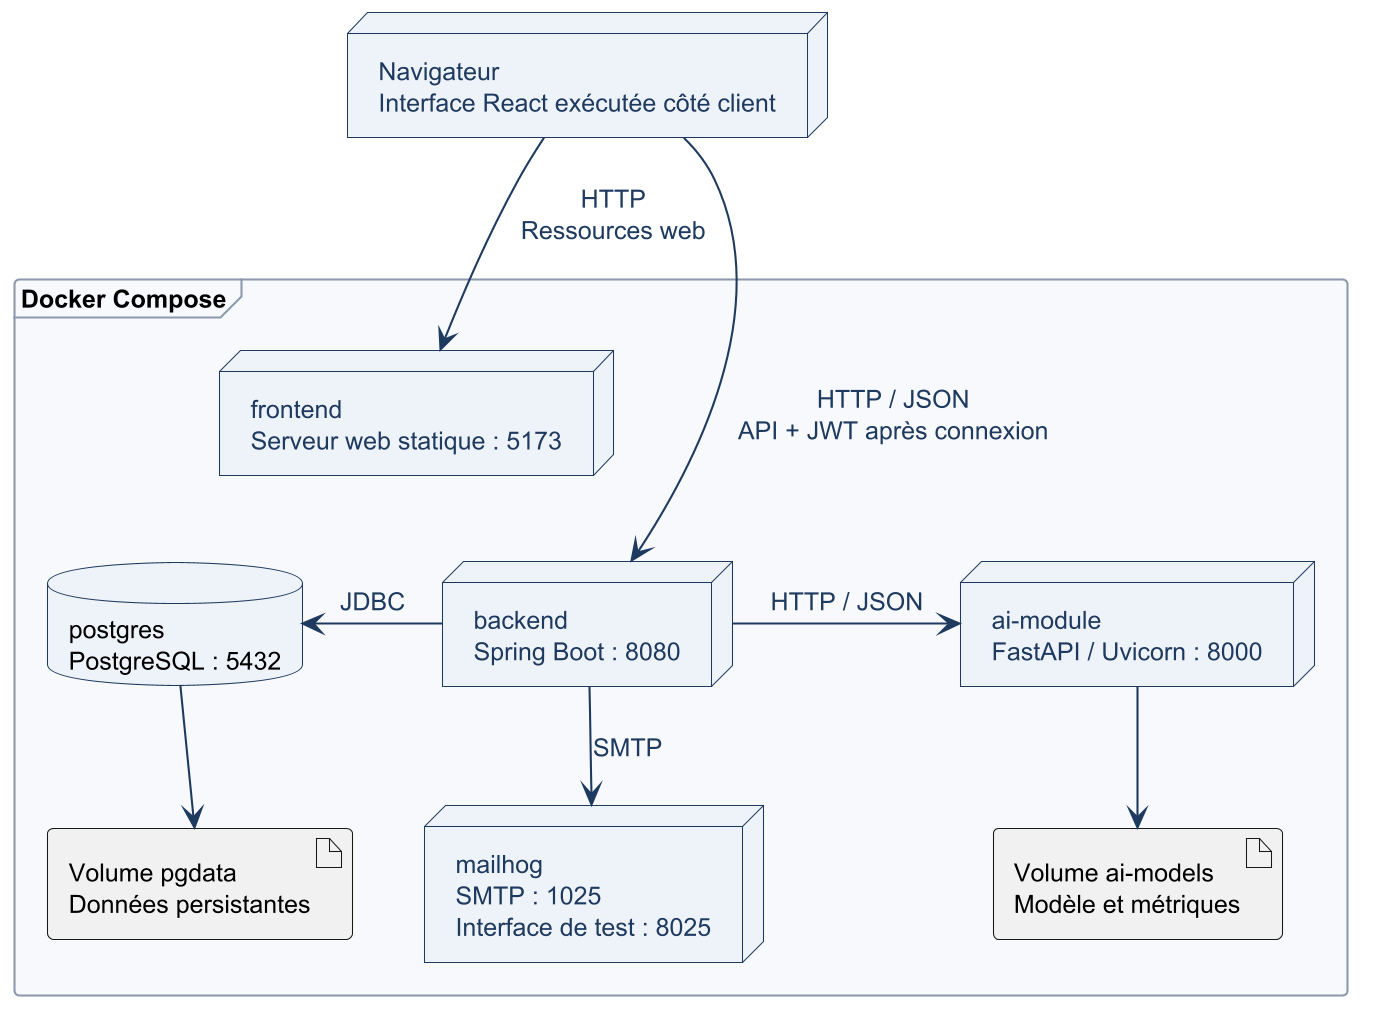
\includegraphics[width=0.95\textwidth,height=0.45\textheight,keepaspectratio]{fig3_2_deploiement_local}
\caption{Déploiement local et principaux protocoles d'échange}
\label{fig:deploiement-local}
\end{figure}

Deux volumes conservent les données utiles : le premier celles de PostgreSQL, le second le modèle d'IA réentraîné et ses métriques. Un redémarrage ou une reconstruction des conteneurs ne fait donc perdre ni les fiches ni les fichiers, point vérifié par la recette. L'ensemble se lance par une seule commande, \texttt{docker compose up -{}-build}, et les adresses d'accès sont celles du tableau~\ref{tab:services}.

\subsection{Portée du déploiement}

Cette configuration vise le développement, la démonstration et la recette. Elle n'est pas un déploiement de production : les paramètres sensibles (secret de signature des jetons, accès à la base) y ont des valeurs par défaut de démonstration, la messagerie est une messagerie de test, et la plateforme ne dispose ni de supervision continue ni de sauvegarde planifiée. Ces points relèvent des perspectives.

\section{Documentation interactive de l'API}

Le backend expose sa description au format OpenAPI et une interface Swagger UI (figure~\ref{fig:swagger}). Cette interface liste les points d'accès, regroupés par domaine, avec leurs paramètres et leurs réponses, et permet de les essayer en fournissant le jeton obtenu à la connexion. La description générée recense cinquante-deux chemins. Elle sert aux développeurs et à la recette ; elle ne constitue pas une interface destinée aux utilisateurs finaux. Le service d'IA fournit de la même façon sa propre documentation, qui décrit le contrat d'échange présenté au chapitre~\ref{ch:sprint4}.

\begin{figure}[H]
\centering
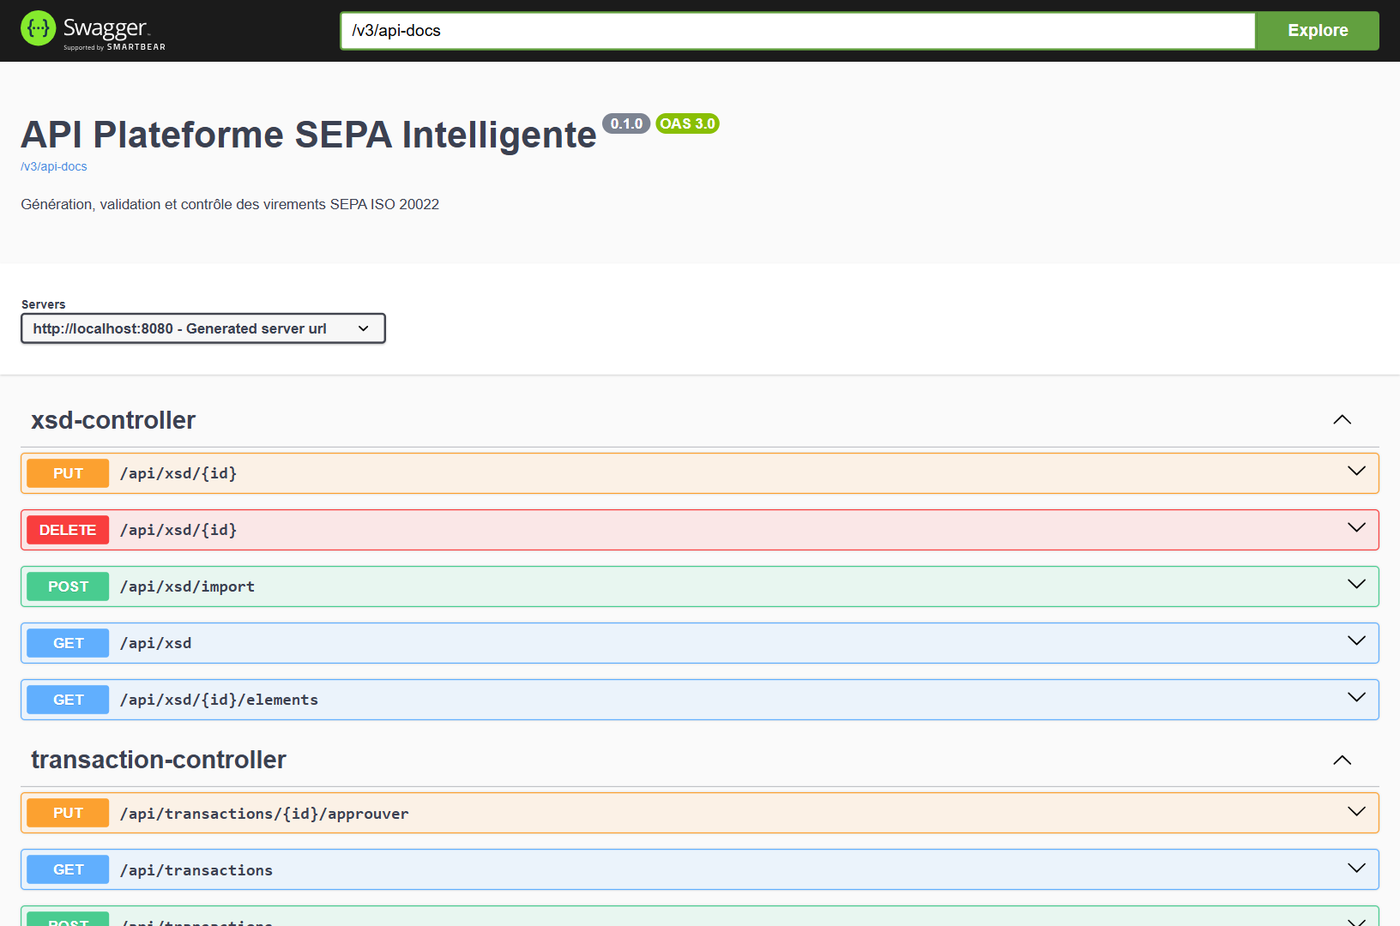
\includegraphics[width=0.9\textwidth]{fig8_swagger}
\caption{Documentation interactive de l'API du backend}
\label{fig:swagger}
\end{figure}

\section{Recette de bout en bout}

\subsection{Démarche}

Les tests automatisés de chaque sprint vérifient les composants un à un. La recette poursuit un autre but : vérifier, sur l'application \textbf{réellement déployée} par Docker Compose, que les parcours complets fonctionnent et que les règles de sécurité tiennent lorsqu'on les traverse comme un utilisateur. Un script rejoue ces parcours par l'API, avec les comptes de démonstration, en passant par l'authentification à double facteur : le code à usage unique est lu dans la messagerie de test, comme le ferait un utilisateur. Chaque vérification compare un résultat attendu à un résultat observé. Le script s'appuie sur le scénario de démonstration du chapitre~\ref{ch:sprint4} (1\,100 fiches pour une société) et le retire une fois la recette terminée.

\subsection{Résultats}

Les quarante vérifications réussissent. Le tableau~\ref{tab:recette} les regroupe par domaine.

\begin{table}[H]
\centering
\footnotesize
\renewcommand{\arraystretch}{1.12}
\tablestyle
\begin{tabularx}{\textwidth}{|>{\raggedright\arraybackslash}p{3.1cm}|Y|>{\centering\arraybackslash}p{1.2cm}|}
\hline
\rowcolor{appMarine}\entete{Domaine} & \entete{Comportements vérifiés} & \entete{Cas} \\
\hline
Authentification & Code exigé après un mot de passe correct, sans jeton émis ; code erroné et mot de passe erroné refusés ; jeton émis avec le bon code ; accès sans jeton refusé & 5 \\
\hline
Droits des profils & Administrateur sans accès aux fiches, avec une supervision sans matricule ; Manager sans accès au journal d'audit ; Expert RH ne pouvant ni créer une société ni approuver une fiche & 7 \\
\hline
Périmètre par société & Un Expert RH ne voit que les fiches et anomalies de ses sociétés (5 fiches contre 9 pour le Manager ; 3 anomalies contre 7) ; sans société affectée, il ne voit rien & 3 \\
\hline
Fiches de paie & Société obligatoire à la saisie ; société non affectée refusée ; fiche à IBAN invalide conservée en brouillon et approbation refusée ; fiche valide approuvée & 5 \\
\hline
Flux de masse & Mille cent paiements listés et contrôlés ; soumission refusée en présence d'une erreur métier ; contrôle après exclusion de la fiche en erreur ; téléchargement préfixé avant validation et au nom d'origine après ; Expert RH sans droit de valider ; rejet sans motif refusé ; double validation refusée & 11 \\
\hline
Indicateurs & Fichiers générés et validés comptés ; indicateurs de l'Expert RH limités à sa société ; société non affectée refusée ; indicateurs d'apport de l'IA disponibles & 4 \\
\hline
Résilience & Module d'IA arrêté : le contrôle aboutit et l'IA est déclarée indisponible ; la supervision le signale ; après redémarrage, l'IA est de nouveau disponible & 3 \\
\hline
Persistance & Données conservées après un redémarrage du backend & 1 \\
\hline
Documentation & Interface et description OpenAPI accessibles, cinquante-deux chemins & 1 \\
\hline
\rowcolor{appClair}\textbf{Total} & & \textbf{40} \\
\hline
\end{tabularx}
\caption{Résultats de la recette de bout en bout}
\label{tab:recette}
\end{table}

Plusieurs mesures méritent d'être commentées. Le contrôle de mille cent paiements, qui comprend les règles métier, l'analyse par l'IA, la génération du XML et la validation XSD, aboutit en quelques secondes : de trois à neuf secondes selon les exécutions, avec neuf fiches signalées par l'IA et un fichier conforme. L'arrêt du module d'IA donne le résultat attendu par la conception du chapitre~\ref{ch:sprint4} : le contrôle aboutit en environ six secondes, le fichier est conforme au schéma, et le résultat indique que l'IA n'a pas été exécutée, ce qui évite de confondre absence d'analyse et absence de risque. Enfin, après redémarrage du backend, les onze fichiers de la recette sont toujours présents.

\subsection{Anomalies décelées par la recette}

La recette a aussi joué son rôle de détecteur. Deux écarts entre le comportement réel et celui décrit dans ce rapport ont été corrigés au cours de ce travail. Le premier, évoqué plus haut, concerne l'étendue du périmètre de l'Expert RH, qui ne s'appliquait pas à la liste des fiches ni aux anomalies. Le second, mis en évidence au chapitre~\ref{ch:sprint3}, concernait un fichier contenant une erreur de contrôle métier, qui pouvait encore être soumis : la soumission est désormais refusée. Ces corrections sont couvertes par des tests automatisés et par la recette.

\section{Bilan quantitatif}

Le tableau~\ref{tab:bilan} résume l'état du projet à l'issue du dernier sprint.

\begin{table}[H]
\centering
\footnotesize
\renewcommand{\arraystretch}{1.12}
\tablestyle
\begin{tabularx}{\textwidth}{|>{\raggedright\arraybackslash}p{5.5cm}|Y|}
\hline
\rowcolor{appMarine}\entete{Élément} & \entete{Résultat} \\
\hline
Tests automatisés du backend & 178 tests, tous réussis \\
\hline
Tests automatisés du module d'IA & 27 tests, tous réussis \\
\hline
Recette de bout en bout & 40 vérifications sur 40 réussies \\
\hline
Chemins documentés de l'API & 52 \\
\hline
Services conteneurisés & 5, lancés par une seule commande \\
\hline
Récits utilisateur du backlog & 24, répartis sur cinq sprints \\
\hline
\end{tabularx}
\caption{Bilan quantitatif du projet}
\label{tab:bilan}
\end{table}

Ces chiffres attestent d'une base vérifiée, sans suffire à garantir l'absence de défaut : le nombre de tests ne mesure pas à lui seul la qualité d'une solution.

\section{Conclusion}

Le sprint 5 a transformé un ensemble de fonctions en plateforme exploitable. Chaque profil dispose d'un tableau de bord orienté action et d'indicateurs définis sans ambiguïté, dont la lecture respecte le cloisonnement des rôles. L'ensemble se déploie par une commande unique, avec un ordre de démarrage maîtrisé et des données conservées. La recette de bout en bout confirme le fonctionnement des parcours, la tenue des règles de sécurité et la résilience face à l'indisponibilité du module d'IA, mais elle porte sur des données de démonstration, dans un environnement de développement, et ne remplace ni un test de charge ni un audit de sécurité.
